\documentclass[english]{article}
\usepackage[T1]{fontenc}
%\usepackage[latin9]{inputenc}
%\usepackage{geometry}
%\geometry{verbose,tmargin=1in,bmargin=1in,lmargin=1in,rmargin=1in}
\usepackage{amsmath}
\usepackage{amssymb}
\usepackage{setspace}
\usepackage[utf8]{inputenc}
\usepackage{graphicx}
\usepackage{float}
\usepackage{adjustbox}
\usepackage{gensymb}
\usepackage{amssymb}
\usepackage{array}
\usepackage{ragged2e}
\usepackage{lipsum}
\onehalfspacing
\usepackage{babel}
\usepackage{ctable}
\usepackage{booktabs}
\usepackage{graphicx}
\usepackage{caption}
\usepackage{placeins}
\usepackage{todonotes}
\usepackage{subcaption}
\usepackage[font=footnotesize,labelformat=simple]{subcaption}
\usepackage[T1]{fontenc}
\usepackage{pdflscape}

\begin{document}

\title{Informality in LAC: Heterogeneity and Disappointing Progress}
\maketitle
\begin{abstract}
    This descriptive paper uses household and employment surveys from the Latin America and the Caribbean region to paint a more complete picture of the different aspects of informality. We start by discussing alternative informality measures at the regional and cross country level. We then show that there has been progress on increasing the share of dependent workers who contribute to social security but that the productive structure of the economies in the region has remained mostly unchanged. We argue that this is mainly coming from the focus of governments policies on facilitating the registration of low productivity workers, therefore subsidizing low productivity firms. To make this point we use two approaches: a qualitative approach based on the analysis of policies that have been identified as successful in reducing informality. Second, we use a simple decomposition on different formalization margins to show that the formalization process in the region has been dominated by workers transitioning to formal status in the same type of firm. This means that the progress made in formalizing workers has happened mainly through increasing coverage of workers in small firms. 
\end{abstract}
\section{Introduction}
\begin{itemize}
    \item Motivation: Informality is a pervasive problem in the region despite many attempts to curtail it. The discussion around informality has been     \item What is informality? 
    
    The mainstream measure of informality comes from the ILO and is interested in following and comparing phenomena that are related but different. 
    \begin{itemize}
        \item Low productivity
        \item Unprotected workers
        \item Unlawful employment
    \end{itemize}
   This paper is divided in two sections the first section looks under the hood of the mainstream informality definition, studies the evolution of alternative measures trying to characterize different segments of informality, document the progress made in reducing informality in the region in the last two decades and their different margins. The second section goes over a summary of the reforms that have been implemented in the region with the goal of reducing informality. 
\end{itemize}
\section{Complexity of Informality}
\begin{itemize}
    \item Mention the history of the term and related literature: Harris Todaro 1970, De Soto, Perryet. al. Ulyssea 2017
 
    \item The mainstream definition of informality comes from the ILO (include the matrix showing the definition of informality). Check the documents coming out of the statistical meeting where they define informality and try to get the concerns behind. 
    \item Include a disaggregation of the different types of ILO informality ( prior: social security explains most of the informal)
       \item International organization have produce many flagship reports on informality : incluir OECD, WB 2021 shadow economy, ILO , IDB, etc. 
       \item the regional discussion has constantly portrayed informality as a public enemy.  
    \item In the next section we look separately at the different components of informality and relate each component with the main policy concern that explains...
\end{itemize}

\section{Labor Market Structure of the Average LAC Country}
Figures \ref{fig:labmarket1} and \ref{fig:labmarket2} shows the structure of the labor market for the average latin american country. 
\begin{itemize}
    \item Structure of the labor market 
    
\begin{figure}[!htb]
\justifying
  \caption{Demographic profile and structure of labor market}
\begin{subfigure}{.9\textwidth}
  \centering
    \subcaption{Demographic}
  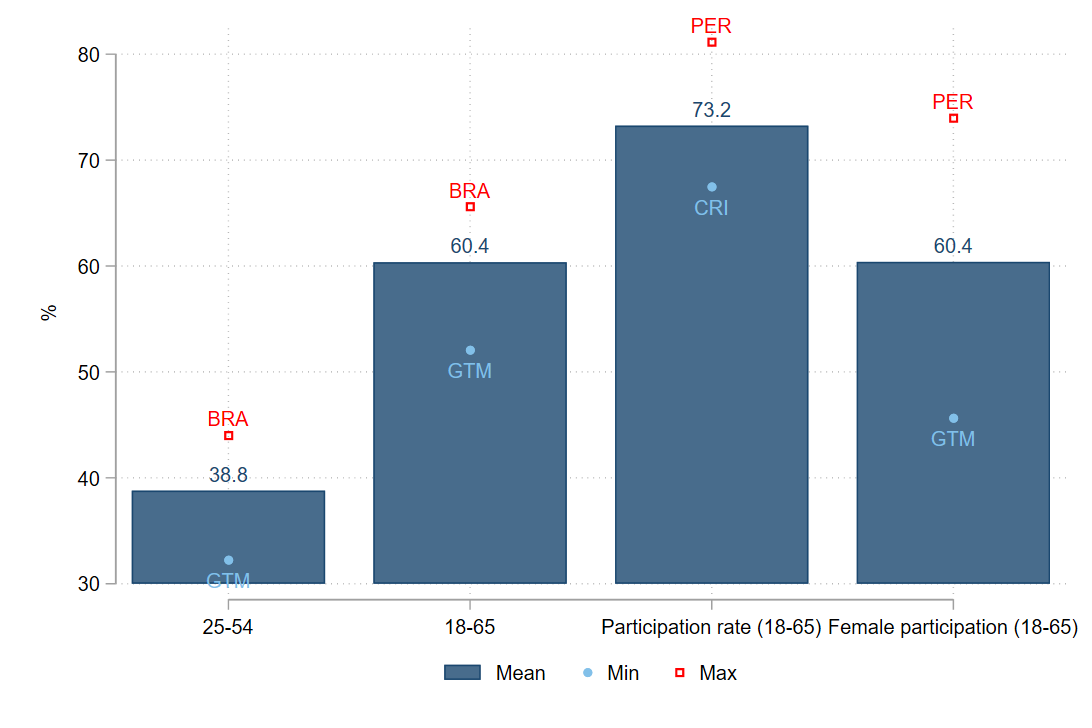
\includegraphics[width=1\linewidth]{latex/figures/Snapshot/Structure of labor market_a.png}
  \label{fig:labmarket1}
\end{subfigure}

\begin{subfigure}{.9\textwidth}
  \centering
    \subcaption{Labor market}
  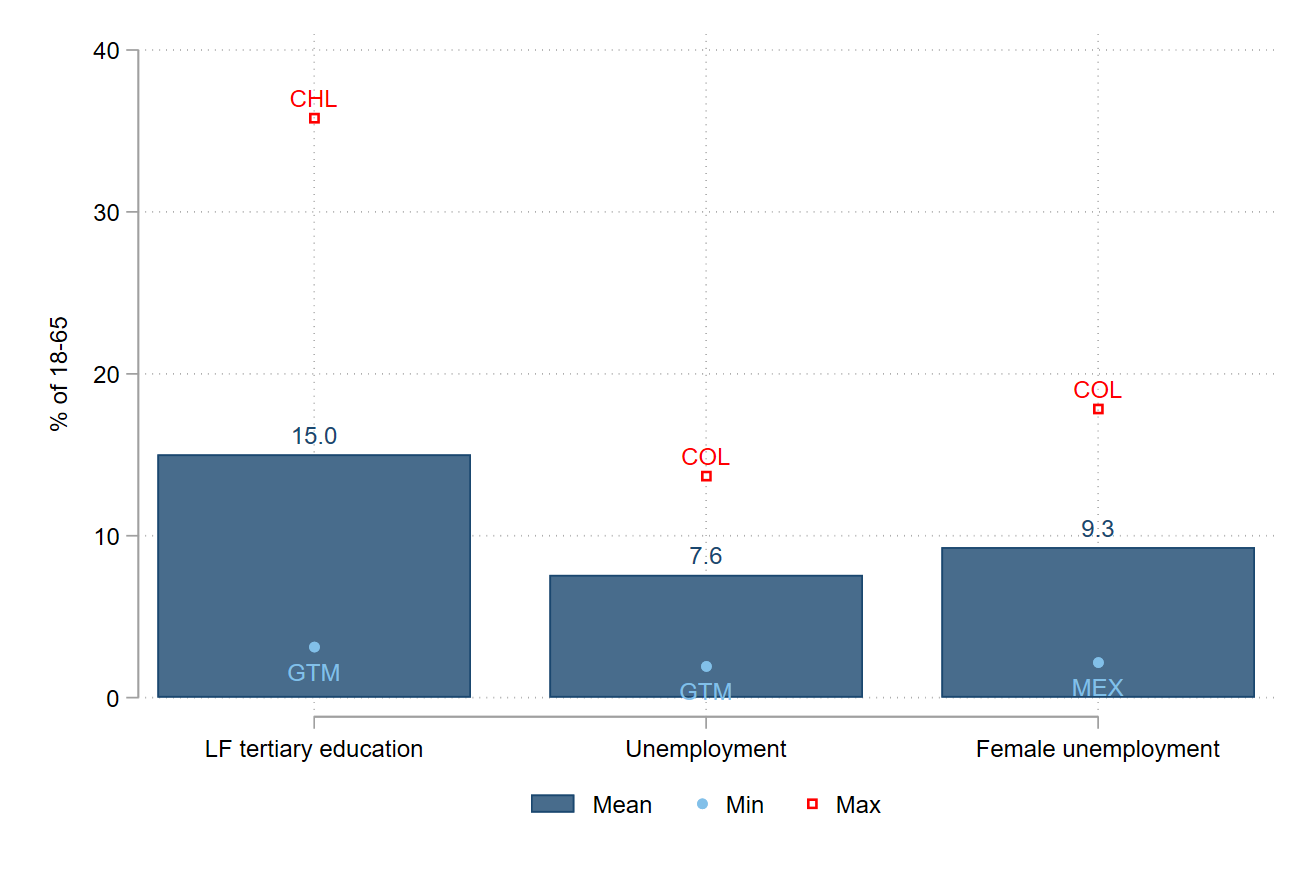
\includegraphics[width=1\linewidth]{latex/figures/Snapshot/Structure of labor market_b.png}
  \label{fig:labmarket2}
\end{subfigure}

\footnotesize{Source: Household Surveys-SEDLAC.}
\footnotesize{Note: Each bar is a simple average of country level weighted average in 2021. Countries included in the sample: Argentina, Bolivia, Brazil, Chile, Colombia, Costa Rica, Dominican Republic, Ecuador, El Salvador, Guatemala, Honduras, Mexico, Panama, Peru, Paraguay and Uruguay. Some countries don’t have information for 2021, in that cases we use the last available year, for Chile 2022, Guatemala 2014; Honduras 2019; Mexico 2018 and Uruguay 2019. Panel a: bar one and two are defined as percentage of the population. Also, "Participation rate" and "Female participation" are define as part of the labor force defined for people between 18 and 65 years old. Panel b: "LF tertiary education" corresponds to people in the workforce who have completed tertiary education.}

\end{figure}
  
    \item Structure of Employment
    
        \begin{figure}[!htb]
        \justifying
        \caption{Structure of employment}     
        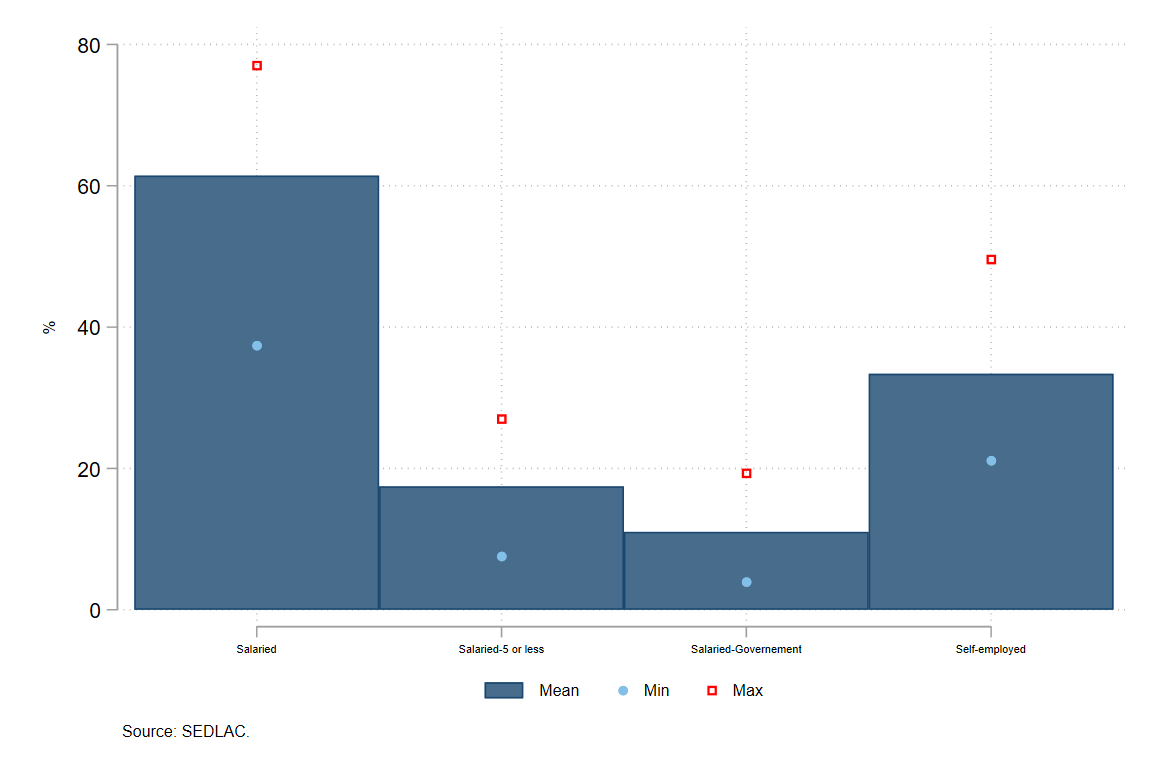
\includegraphics[scale=.3]{latex/figures/Snapshot/Structure of employment.png}
        \label{fig:employment}
        \footnotesize{Source: Household Surveys-SEDLAC.}
        \footnotesize{Note: Each bar is a simple average of country level weighted average in 2021. Countries included in the sample: Argentina, Bolivia, Brazil, Chile, Colombia, Costa Rica, Dominican Republic, Ecuador, El Salvador, Guatemala, Honduras, Mexico, Panama, Peru, Paraguay and Uruguay. Some countries don’t have information for 2021, in that cases we use the last available year, for Chile 2022, Guatemala 2014; Honduras 2019; Mexico 2018 and Uruguay 2019. The "non-salaried" category corresponds to unpaid workers such as family or cooperative workers.}
        \end{figure}

\begin{figure}[htb!]
\centering
  \caption{Structure of salaried and self-employed workers}
  \subcaption{\textbf{Education level}}
    \begin{subfigure}{.5\textwidth}
  \centering
    \footnotesize{$Salaried$}
  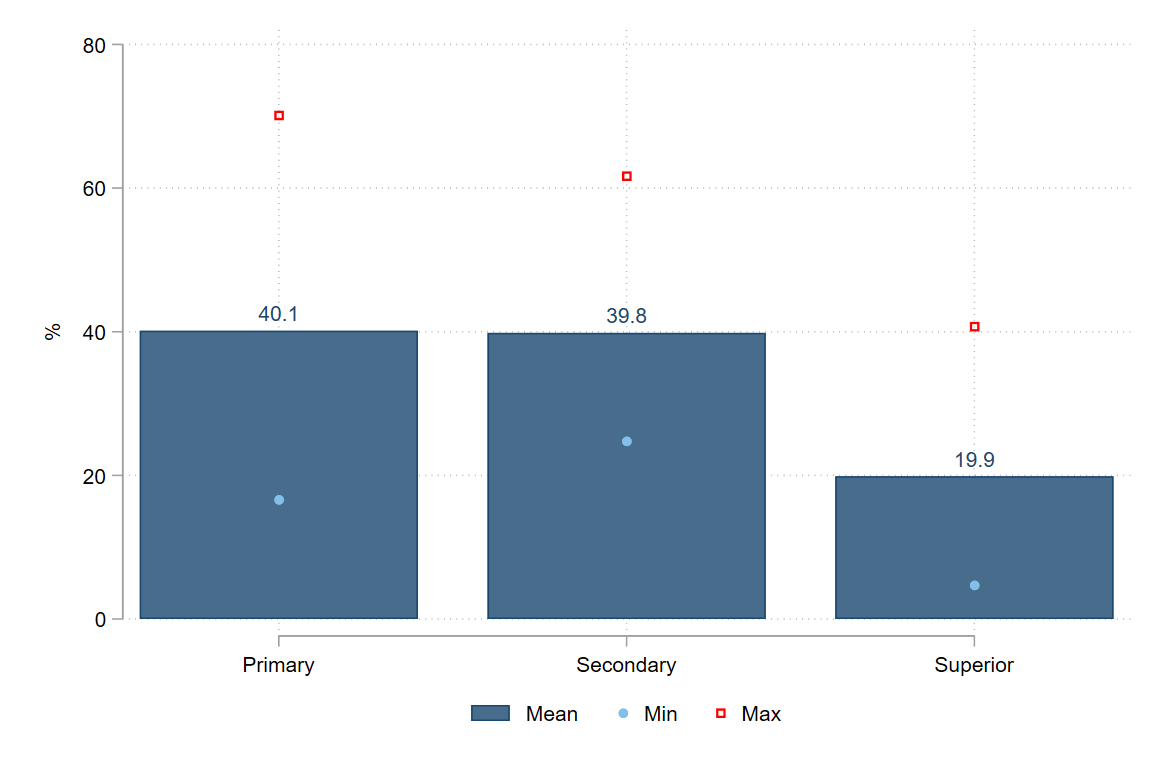
\includegraphics[width=1\textwidth]{latex/figures/Snapshot/Salaried-education.png}
  \label{fig:salariededuc}
\end{subfigure}%
\begin{subfigure}{.5\textwidth}
  \centering
    \footnotesize{$Self employed$}
  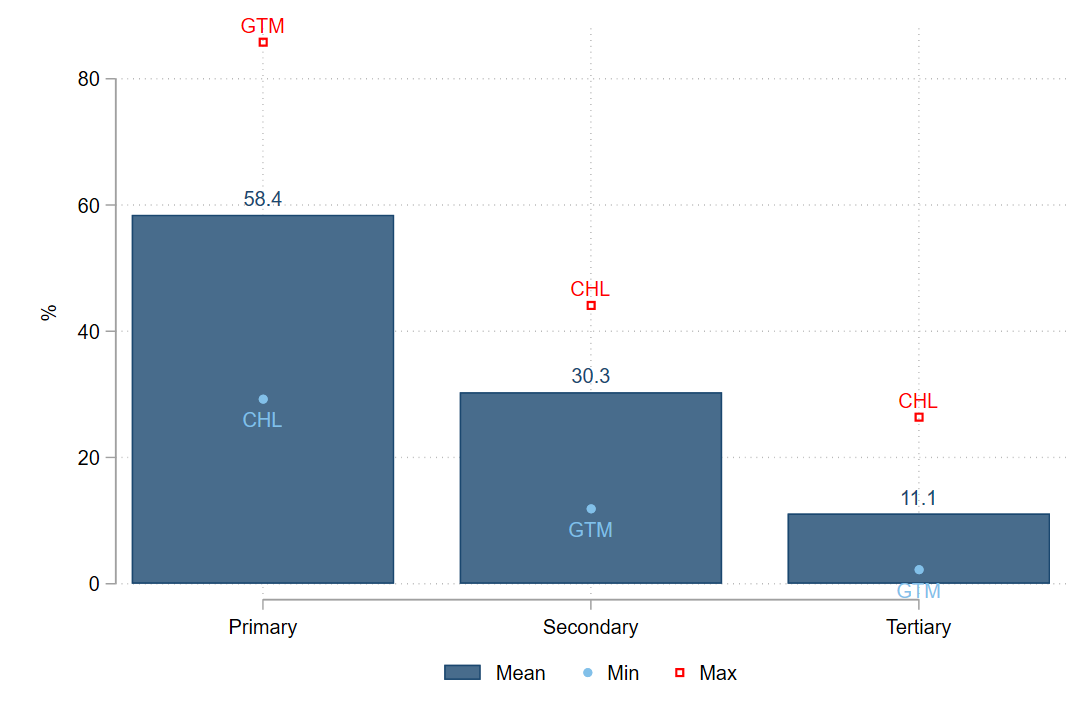
\includegraphics[width=1\textwidth]{latex/figures/Snapshot/Self employed-education.png}
  \label{fig:selfeduc}
\end{subfigure}

\subcaption{\textbf{Firm type}}
\begin{subfigure}{.5\textwidth}
  \centering
    \footnotesize{$Salaried$}
  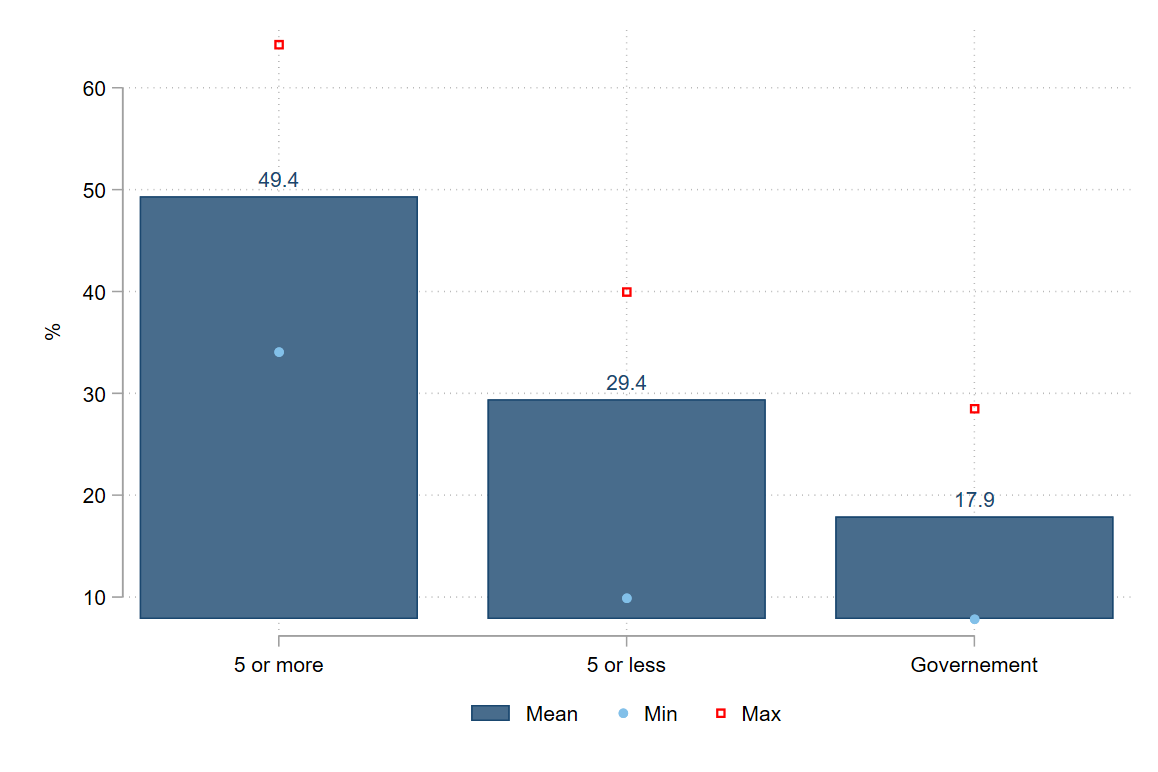
\includegraphics[width=1\textwidth]{latex/figures/Snapshot/Salaried-firmsize.png}
  \label{fig:salariedfirmsize}
\end{subfigure}%
\begin{subfigure}{.5\textwidth}
  \centering
    \footnotesize{$Self employed$}
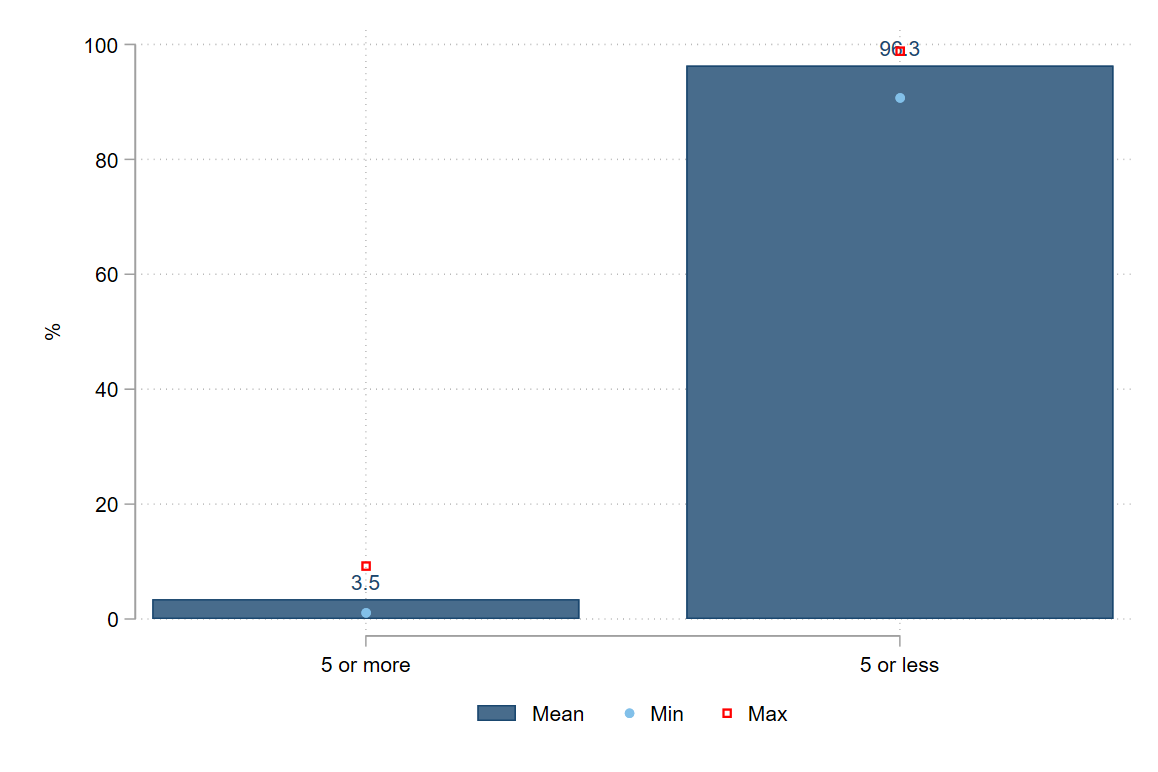
\includegraphics[width=1\textwidth]{latex/figures/Snapshot/Self employed-firmsize.png}
  \label{fig:selfirmsize}
\end{subfigure}

\subcaption{\textbf{Sector}}
\begin{subfigure}{.5\textwidth}
  \centering
  \footnotesize{$Salaried$}
  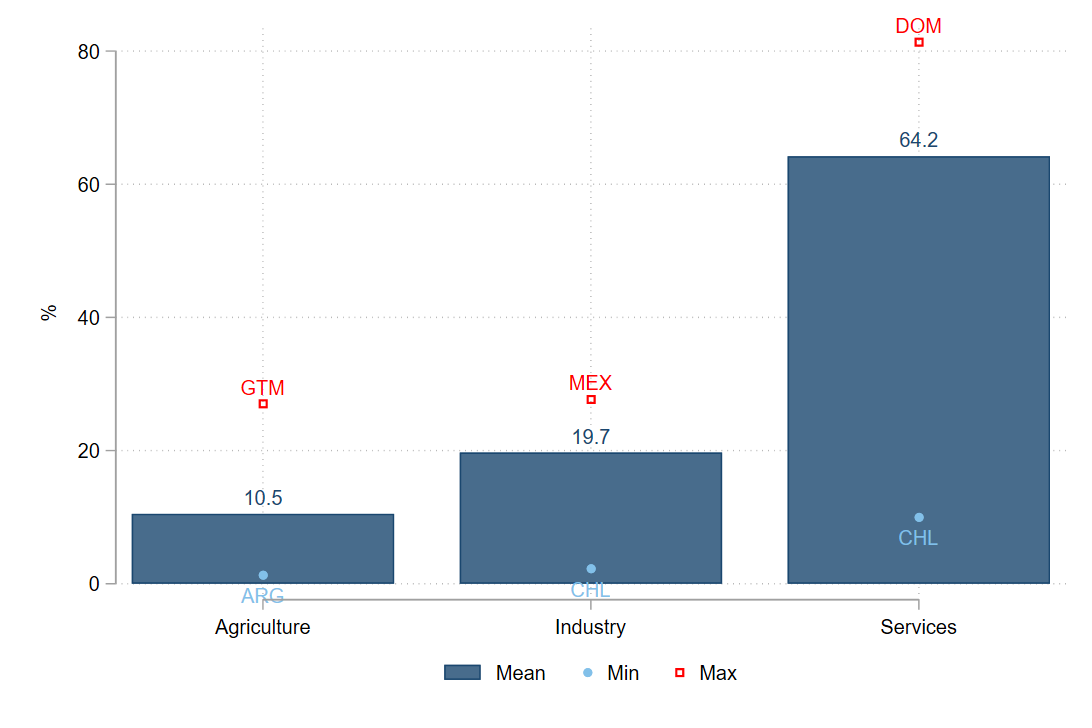
\includegraphics[width=1\textwidth]{latex/figures/Snapshot/Salaried-sector.png}
  \label{fig:salariedsector}
\end{subfigure}%
\begin{subfigure}{.5\textwidth}
  \centering
  \footnotesize{$Self employed$}
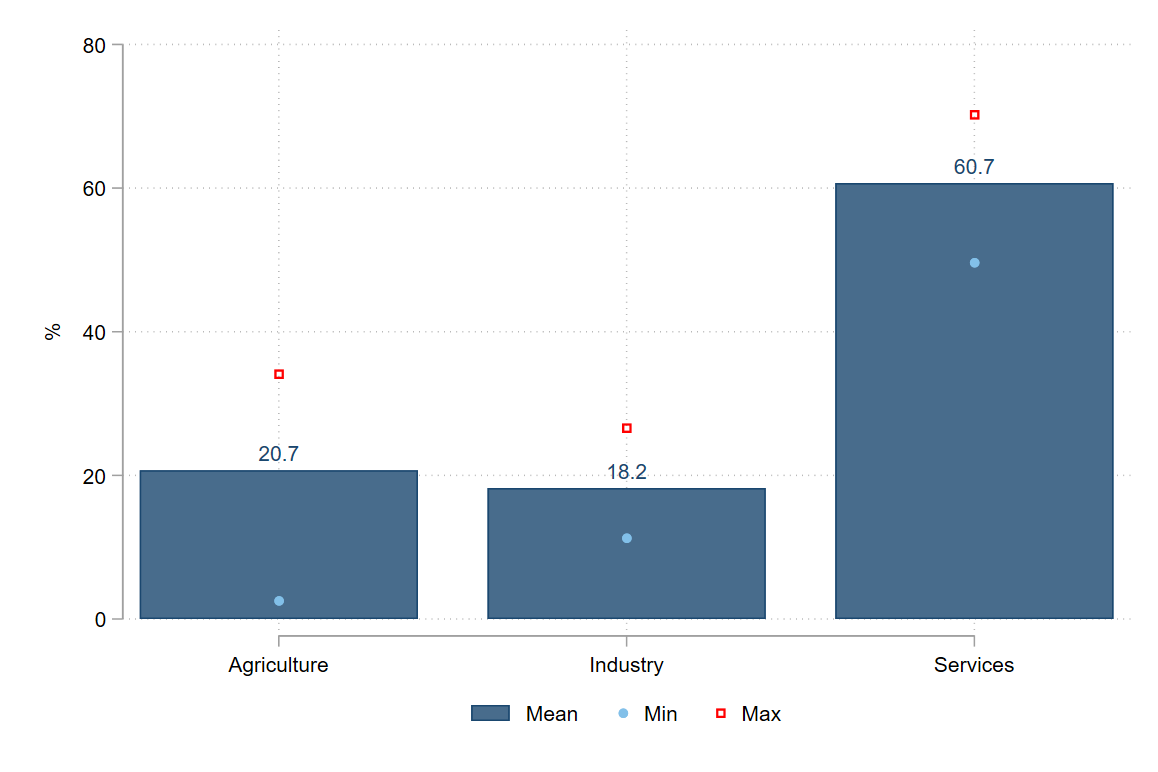
\includegraphics[width=1\textwidth]{latex/figures/Snapshot/Self employed-sector.png}
  \label{fig:selfsector}
\end{subfigure}

\subcaption{\textbf{Contributions to SS}}
\begin{subfigure}{.5\textwidth}
  \centering
    \footnotesize{$Salaried$}
  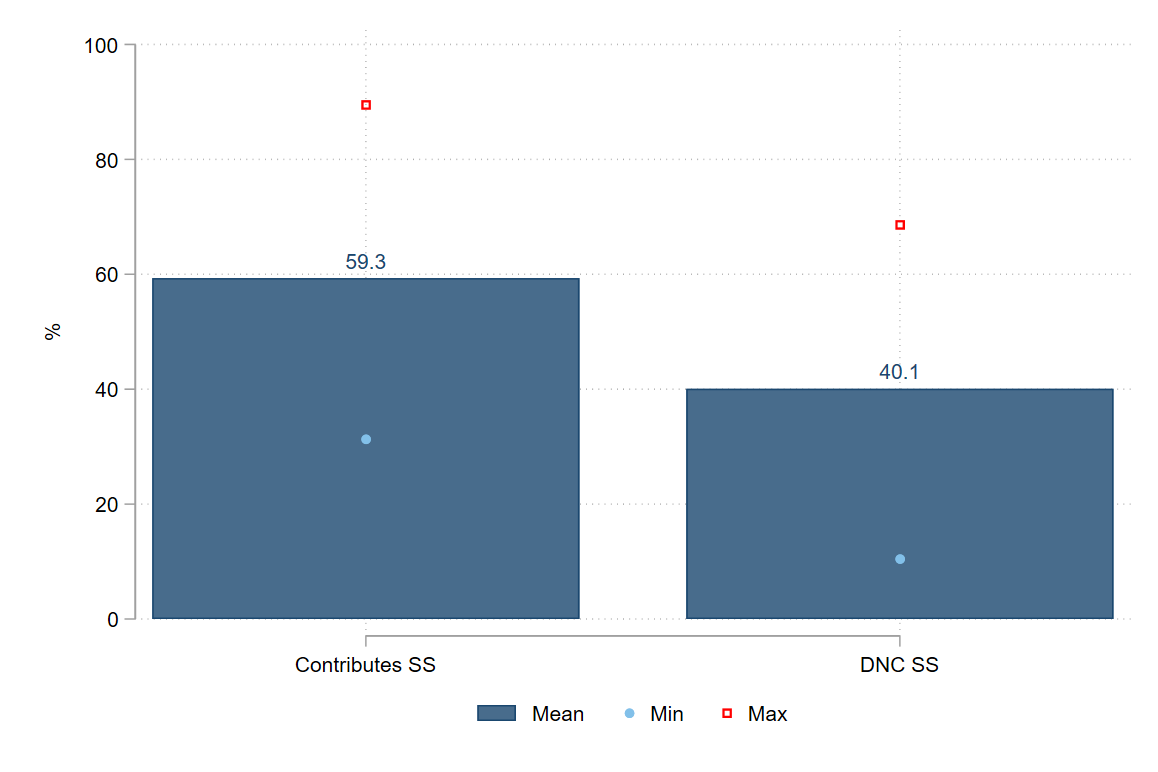
\includegraphics[width=1\textwidth]{latex/figures/Snapshot/Salaried-SS.png}
  \label{fig:salariedSS}
\end{subfigure}%
\begin{subfigure}{.5\textwidth}
  \centering
\footnotesize{$Self employed$}
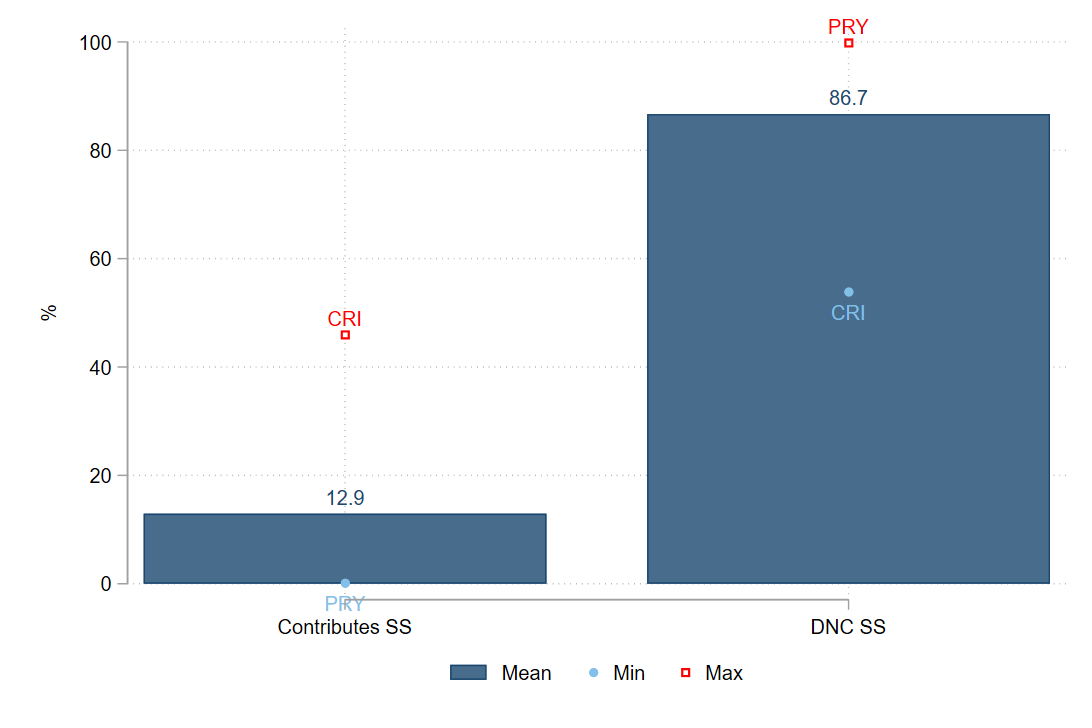
\includegraphics[width=1\textwidth]{latex/figures/Snapshot/Self employed-SS.png}
  \label{fig:selfSS}
\end{subfigure}
\justifying
\footnotesize{Source: Household Surveys-SEDLAC.}
\footnotesize{Note: Each bar is a simple average of country level weighted average in 2021. Countries included in the sample: Argentina, Bolivia, Brazil, Chile, Colombia, Costa Rica, Dominican Republic, Ecuador, El Salvador, Guatemala, Honduras, Mexico, Panama, Peru, Paraguay and Uruguay. Some countries don’t have information for 2021, in that cases we use the last available year, for Chile 2022, Guatemala 2014; Honduras 2019; Mexico 2018 and Uruguay 2019. Argentina and Chile are excluded from contributions to Social security of self-employed graph, because this question is available only for salaried workers. Also, Chile is excluded from calculations of self-employed in sectors, because is only for salaried workers.}

\end{figure}
         

        
\item Structure of Employment II - Sector and Contribution to SS

\begin{figure}[!htb]
        \justifying
        \caption{Structure of employment by sector}     
        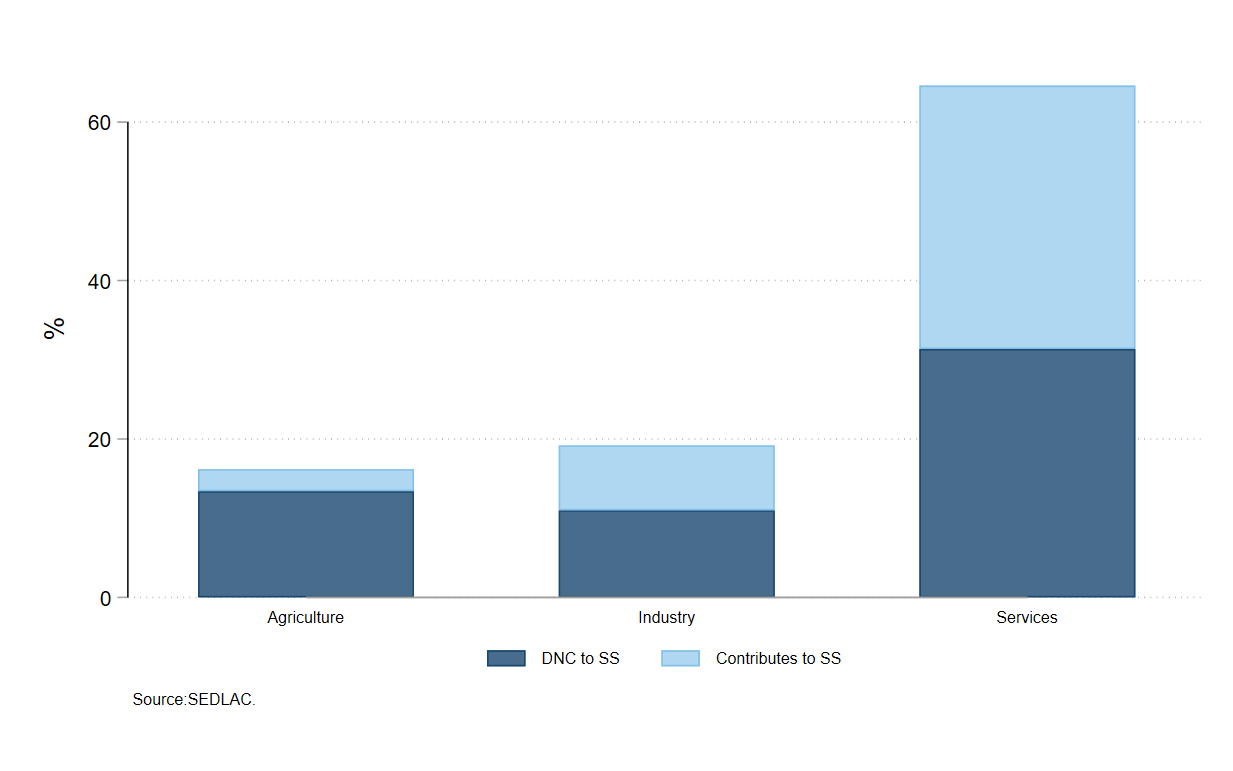
\includegraphics[scale=.3]{latex/figures/Snapshot/Structure of employment and sector.png}
        \label{fig:sector}
       \footnotesize{Source: Household Surveys-SEDLAC.}
        \footnotesize{Note: Each bar is a simple average of country level weighted average in 2021. Countries included in the sample: Bolivia, Brazil, Chile, Colombia, Costa Rica, Dominican Republic, Ecuador, El Salvador, Guatemala, Honduras, Mexico, Panama, Peru, Paraguay and Uruguay. Some countries don’t have information for 2021, in that cases we use the last available year, for Chile 2022, Guatemala 2014; Honduras 2019; Mexico 2018 and Uruguay 2019. Argentina is excluded from this figure because the household survey is urban.}
\end{figure}

        
\item Employment by Firm Size
\begin{figure}[!htb]
        \justifying
        \caption{Structure of private employment by firm size}     
        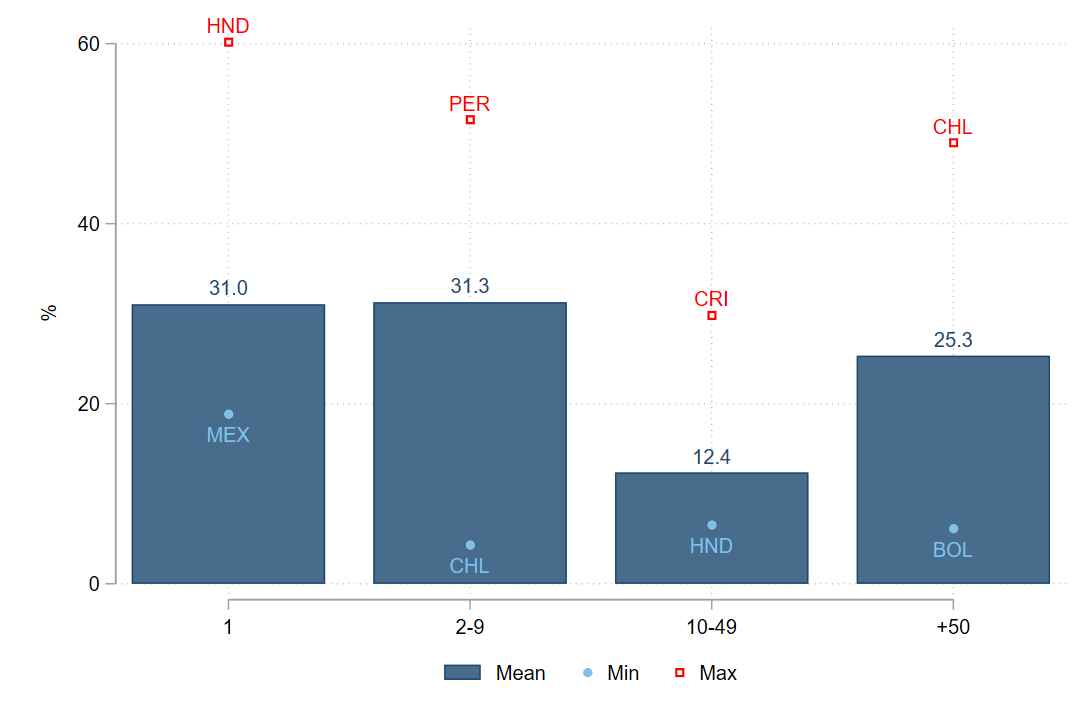
\includegraphics[scale=.3]{latex/figures/Snapshot/Structure of employment by firm size.png}
        \label{fig:firmsize}
        \footnotesize{Source: Household Surveys-SEDLAC.}
        \footnotesize{Note: Each bar is a simple average of country level weighted average in 2021. Countries included in the sample: Bolivia, Brazil, Chile, Colombia, Costa Rica, Ecuador, El Salvador, Honduras, Mexico, Panama, Peru, Paraguay and Uruguay. Some countries don’t have information for 2021, in that cases we use the last available year, for Chile 2022, Guatemala 2014; Honduras 2019; Mexico 2018 and Uruguay 2019. We exclude Argentina, Dominican Republic and Guatemala, because of missing information in firm size variable.}
        \end{figure}


        
 \item Social security contributions
    \begin{itemize}
        \begin{figure}[!htb]
        \justifying
        \caption{Share of Workers Who Do Not Contribute to Social Security by Selected Characteristics}     
        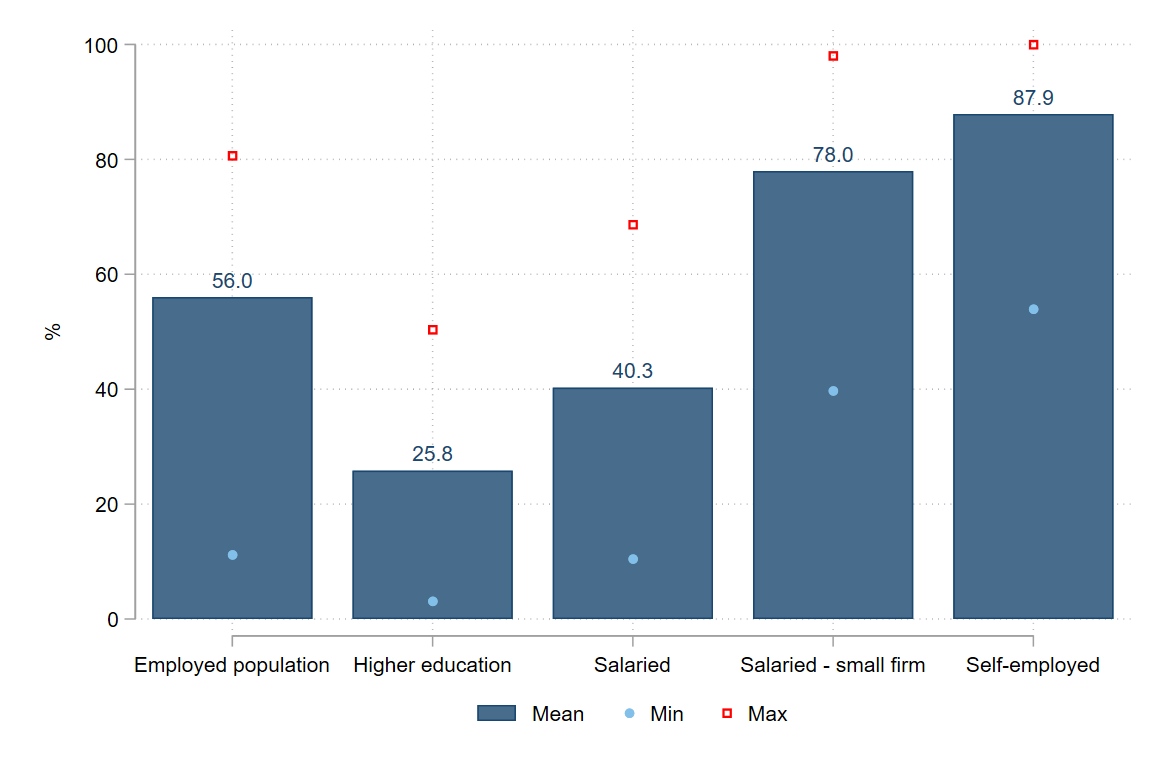
\includegraphics[scale=.3]{latex/figures/Snapshot/Social security contributions.png}
        \label{fig:SScontributions}
        \footnotesize{Source: Household Surveys-SEDLAC.}
        \footnotesize{Note: Each bar is a simple average of country level weighted average in 2021. Countries included in the sample: Argentina, Bolivia, Brazil, Chile, Colombia, Costa Rica, Dominican Republic, Ecuador, El Salvador, Guatemala, Honduras, Mexico, Panama, Peru, Paraguay and Uruguay. Some countries don’t have information for 2021, in that cases we use the last available year, for Chile 2022, Guatemala 2014; Honduras 2019; Mexico 2018 and Uruguay 2019. \textbf{The groups are not exclusive.} "Tertiary education" corresponds to people in the workforce who have completed tertiary level of education. "Salaried-Small firm" are salaried employees that work in a firm of 5 or less workers.}
        \end{figure}


\item Life cycle- self employment and salaried informal
 \begin{figure}[!htb]
        \justifying
        \caption{Age profile}     
        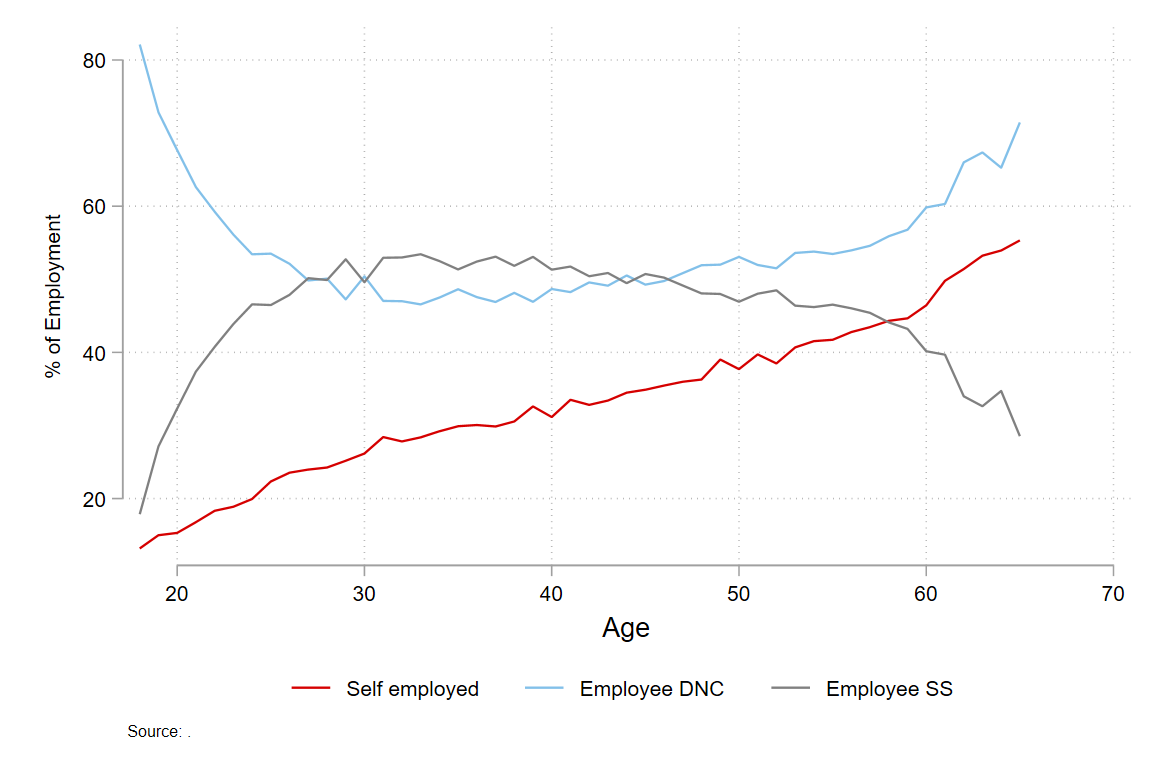
\includegraphics[scale=.3]{latex/figures/Snapshot/age_profile.png}
        \label{fig:age_pro}
        \footnotesize{Source: Household Surveys-SEDLAC.}
        \footnotesize{Note: Each line is a weighted average of countries, weighting by total workers in 2021. Countries included in the sample: Argentina, Bolivia, Brazil, Chile, Colombia, Costa Rica, Dominican Republic, Ecuador, El Salvador, Guatemala, Honduras, Mexico, Panama, Peru, Paraguay and Uruguay. Some countries don’t have information for 2021, in that cases we use the last available year, for Chile 2022, Guatemala 2014; Honduras 2019; Mexico 2018 and Uruguay 2019.}
        \end{figure}
\item Decomposition of changes in the informality rate

\end{itemize}

     
     
\section{Dynamics: last 20 years}  

\subsection{Cross country figures}
\subsubsection{Household}

\begin{figure}[!htb]
    \justifying
     \caption{Snapshot of LAC’s household contribution status}     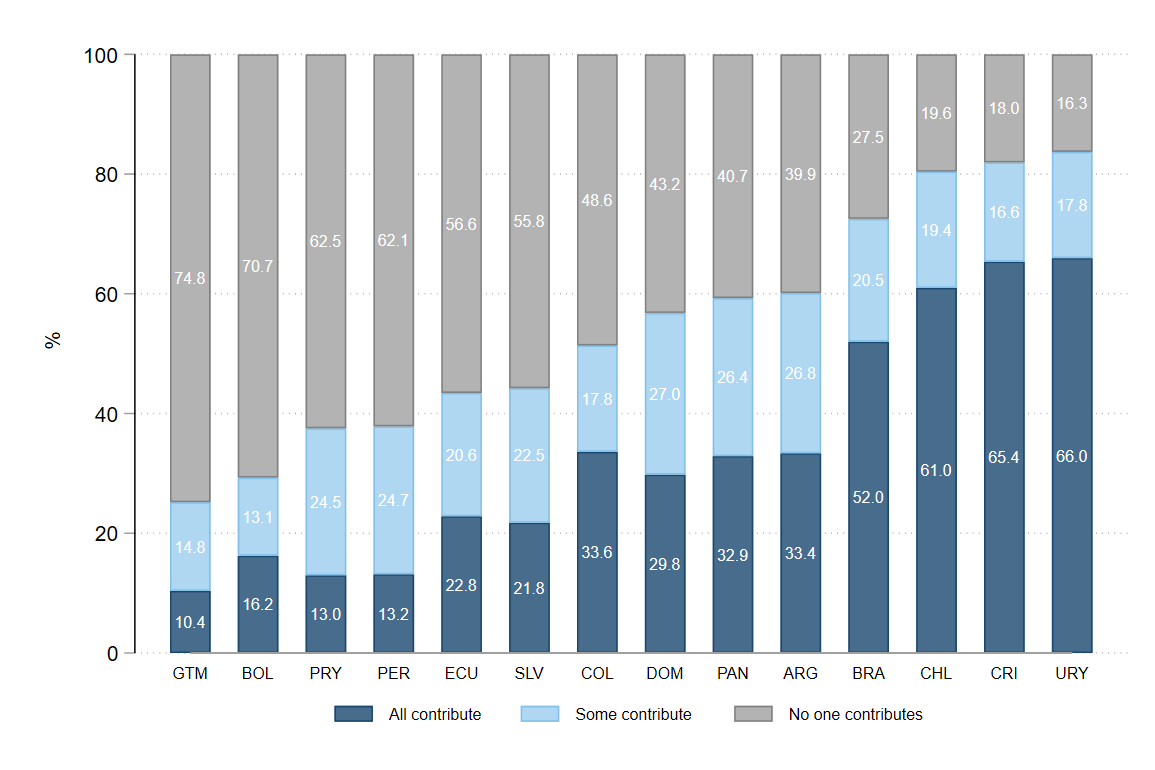
\includegraphics[scale=.3]{latex/figures/Household/snapshot_household.png}
    \label{fig:Householdlastyear}
    \footnotesize{Source: Household Surveys-SEDLAC.}
    \footnotesize{Note: Each bar is a weighted average of each country, weighting by total workers in 2021. Data corresponds to 2021 except for for Chile 2022, Guatemala 2014; Honduras 2019; Mexico 2018 and Uruguay 2019.}
    \footnotesize{Note: The figure reports the household contribution status to social security of households with at least one member works.   All contribute: corresponds to the percentage of households where all workers contribute to SS. Some contribute: corresponds to the percentage of households where some workers contribute to SS but not all. DNC – has partner: corresponds to the percentage of households where any worker contributes to SS, but the head of household have a partner. DNC – no partner: corresponds to the percentage of households where any worker contributes to SS, but the head of household do not have a partner.}
\end{figure}

\subsubsection{Individual level} %De este nombre no estoy segura

\begin{figure}[!htb]
    \justifying
     \caption{Salaried who don’t contribute to SS}     
     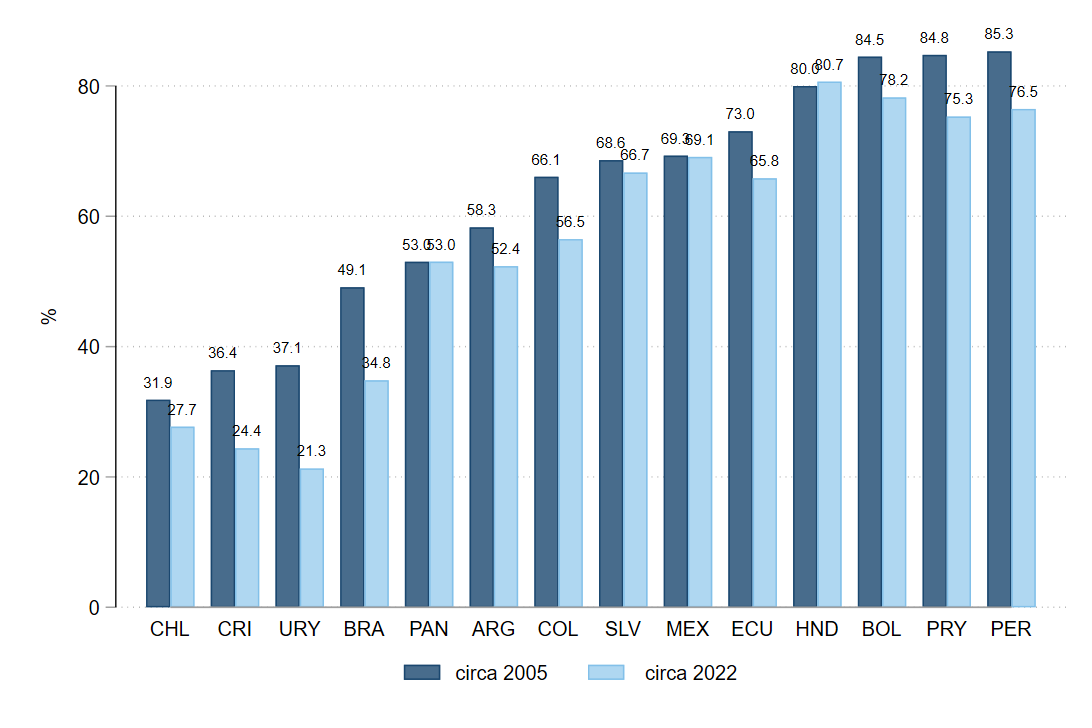
\includegraphics[scale=.3]{latex/figures/Snapshot/snapshot_informal_ss.png}
    \label{fig:SalariedSS}
    \footnotesize{Source: Household Surveys-SEDLAC.}
    \footnotesize{Note: Each bar is a weighted average of each country, weighting by total workers in 2005 and 2021. Countries included in the sample: Argentina, Bolivia, Brazil, Chile, Colombia, Costa Rica, Dominican Republic, Ecuador, El Salvador, Guatemala, Honduras, Mexico, Panama, Peru, Paraguay and Uruguay. Some countries don’t have information for 2021, in that cases we use the last available year, for Chile 2022, Guatemala 2014; Honduras 2019; Mexico 2018 and Uruguay 2019.}
\end{figure}

\begin{figure}[!htb]
    \justifying
     \caption{Salaried who don’t contribute to SS}     
     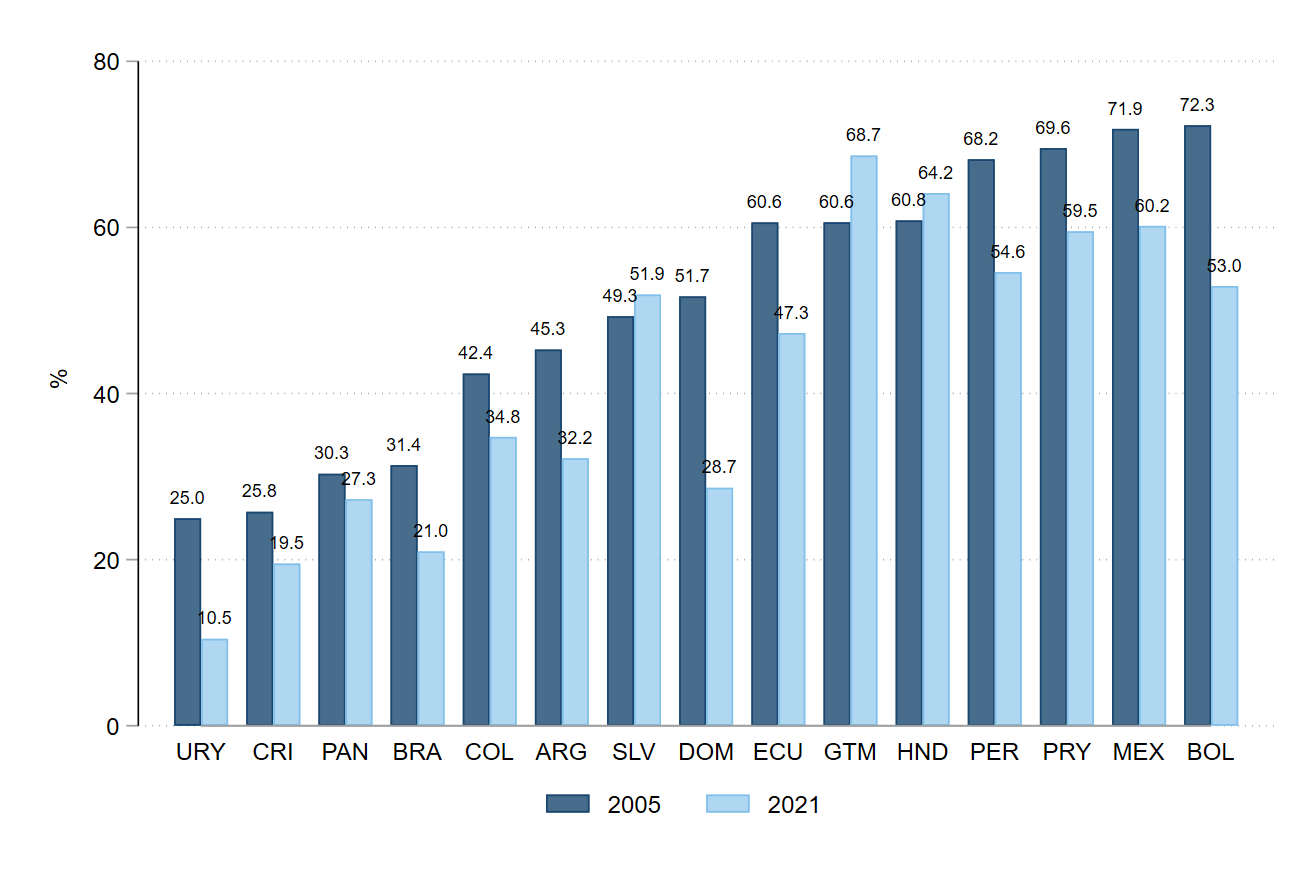
\includegraphics[scale=.3]{latex/figures/Snapshot/snapshot_informal_ss_dep.png}
    \label{fig:SalariedSS}
    \footnotesize{Source: Household Surveys-SEDLAC.}
    \footnotesize{Note: Each bar is a weighted average of each country, weighting by total workers in 2005 and 2021. Countries included in the sample: Argentina, Bolivia, Brazil, Chile, Colombia, Costa Rica, Dominican Republic, Ecuador, El Salvador, Guatemala, Honduras, Mexico, Panama, Peru, Paraguay and Uruguay. Some countries don’t have information for 2021, in that cases we use the last available year, for Chile 2022, Guatemala 2014; Honduras 2019; Mexico 2018 and Uruguay 2019.}
\end{figure}

\begin{figure}[!htb]
    \justifying
     \caption{Salaried who work at small firms}     
     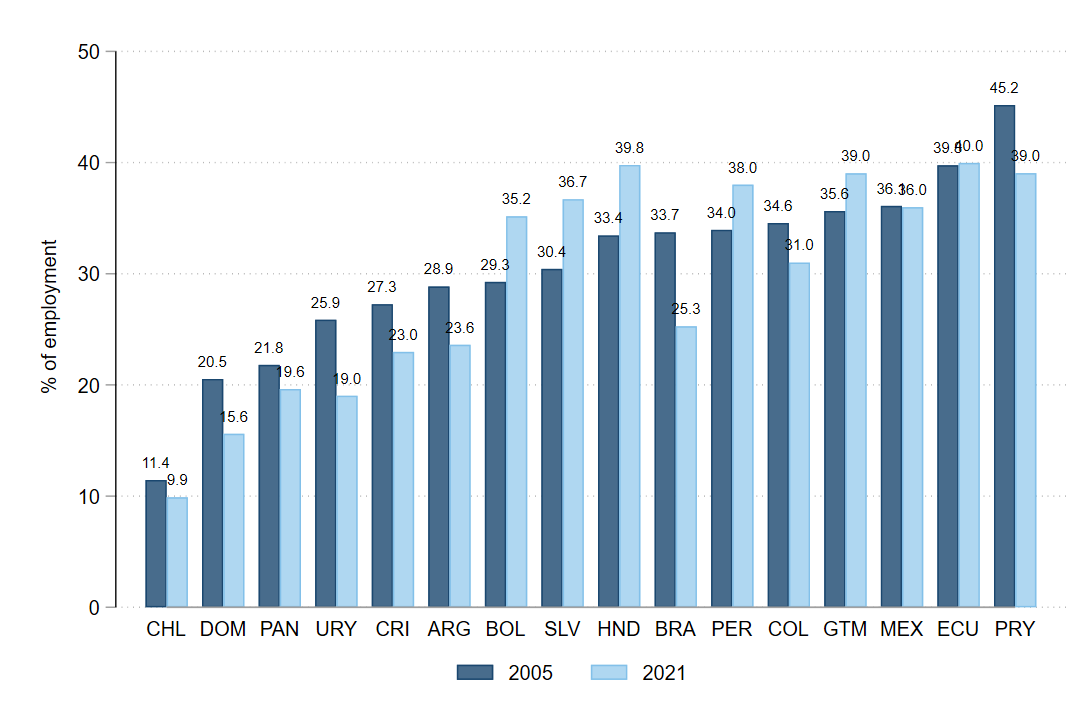
\includegraphics[scale=.3]{latex/figures/Snapshot/snapshot_dependents_small.png}
    \label{fig:SalariedSmall}
    \footnotesize{Source: Household Surveys-SEDLAC.}
    \footnotesize{Note: Each bar is a weighted average of each country, weighting by total workers in 2005 and 2021. Countries included in the sample: Argentina, Bolivia, Brazil, Chile, Colombia, Costa Rica, Dominican Republic, Ecuador, El Salvador, Guatemala, Honduras, Mexico, Panama, Peru, Paraguay and Uruguay. Some countries don’t have information for 2021, in that cases we use the last available year, for Chile 2022, Guatemala 2014; Honduras 2019; Mexico 2018 and Uruguay 2019.}
\end{figure}


\todo[inline]{Check footnote of figure \ref{fig:Oaxaca_share} and make sure the title is correct. Let's include a small appendix with the methodolgy details.}
      

\begin{figure}[!htb]
        \justifying
        \caption{Microeconometric decomposition of evolution of workers who does not contribute to ss 2005-2021}     
        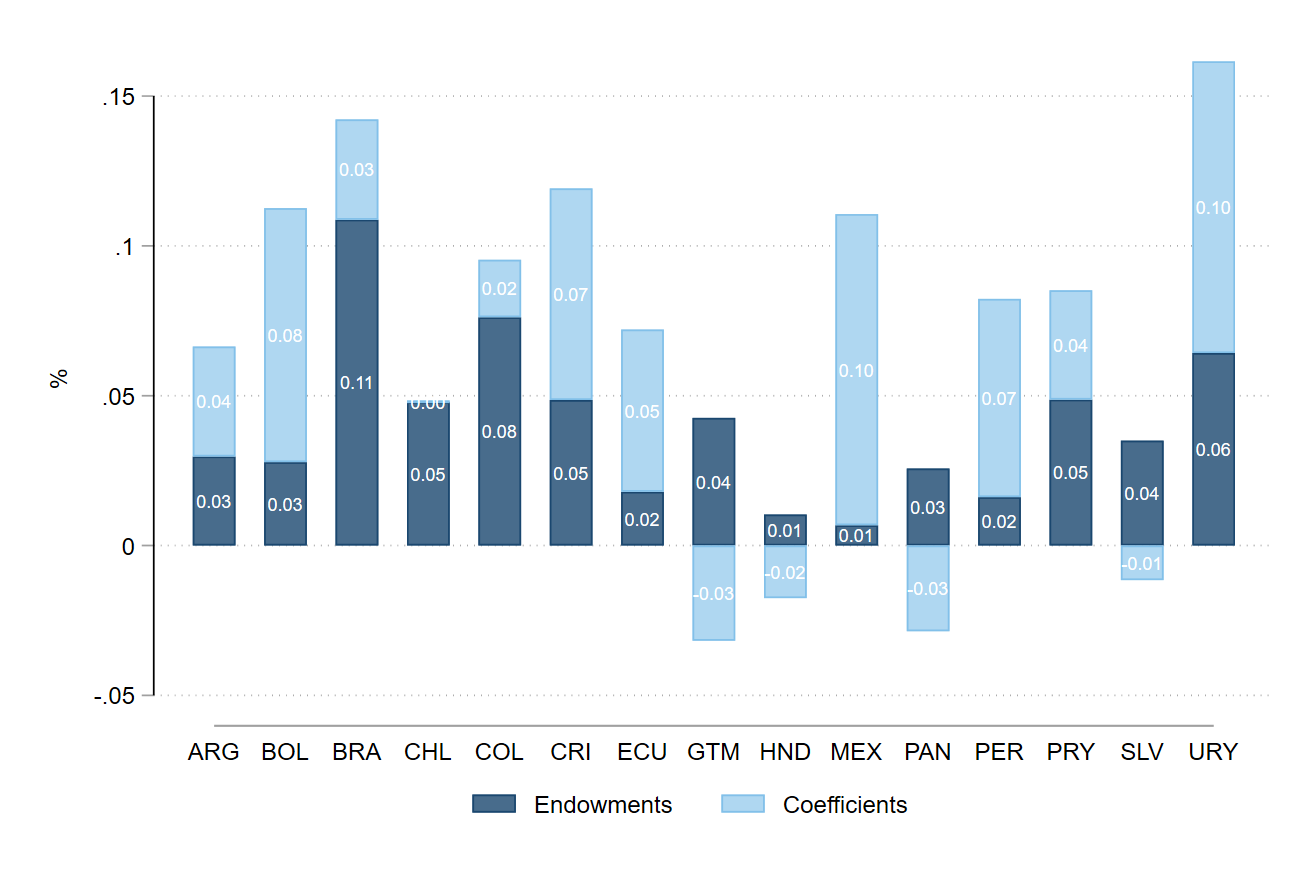
\includegraphics[scale=.3]{latex/figures/Snapshot/Oaxaca decomposition level.png}
        \label{fig:Oaxaca_level}
        \footnotesize{Source: Household Surveys-SEDLAC.}
        \footnotesize{Note: Each bar is the actual change in Social security contributions corresponds to the level of coefficients and the level of the endowment effects. Countries included in the sample: Argentina, Bolivia, Brazil, Chile, Colombia, Costa Rica, Dominican Republic, Ecuador, El Salvador, Guatemala, Honduras, Mexico, Panama, Peru, Paraguay and Uruguay. Some countries don’t have information for 2021, in that cases we use the last available year, for Chile 2022, Guatemala 2014; Honduras 2019; Mexico 2018 and Uruguay 2019.}
        \end{figure}
\end{itemize}

\section{Appendix}

\begin{landscape}
\begin{figure}[!htb]
    \centering
    \caption{Snapshot of LAC’s household employment condition for 2005-2021}     
    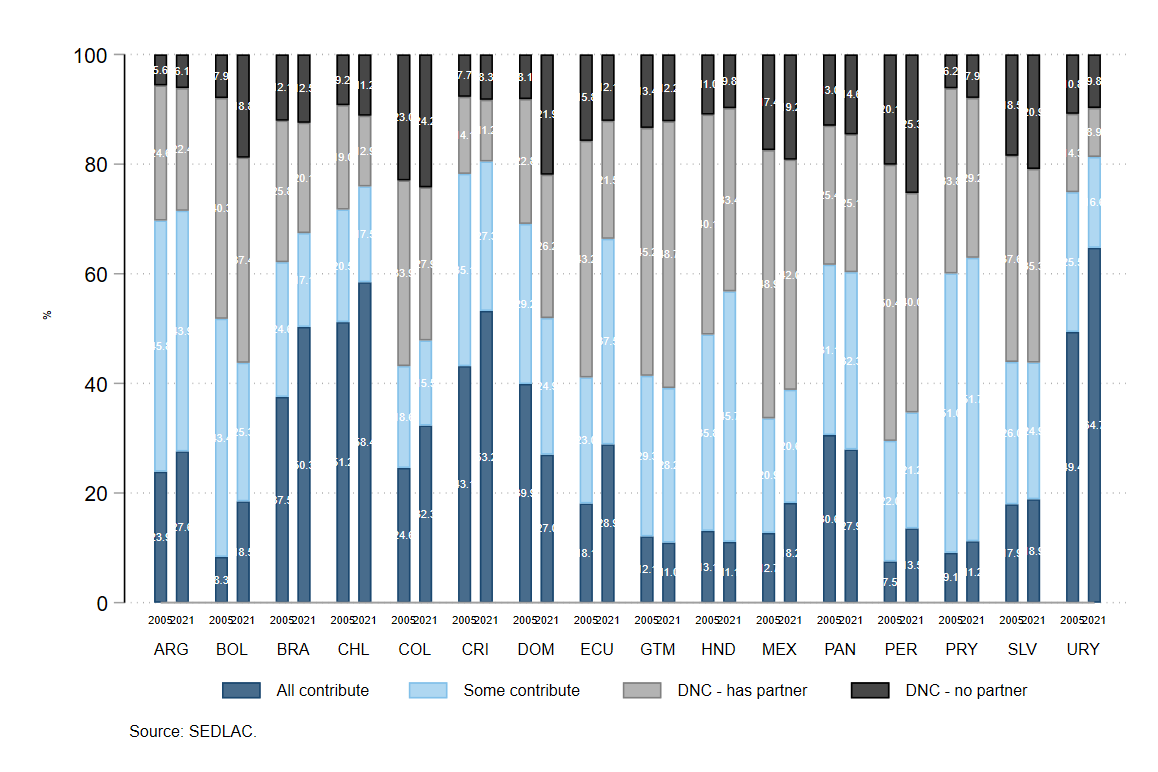
\includegraphics[scale=.45]{latex/figures/Household/snapshot_household_2005-2021.png}
    \label{fig:Household20052021}
    \justifying
    \footnotesize{Source: Household Surveys-SEDLAC.}
    \footnotesize{Note: Each bar is a weighted average of each country, weighting by total workers in 2005 and 2021.Data corresponds to 2021 except for Chile 2022, Guatemala 2014; Honduras 2019; Mexico 2018 and Uruguay 2019.}
    \footnotesize{Note: The figure reports the household contribution status to social security of households with at least one member works.   All contribute: corresponds to the percentage of households where all workers contribute to SS. Some contribute: corresponds to the percentage of households where some workers contribute to SS but not all. DNC – has partner: corresponds to the percentage of households where any worker contributes to SS, but the head of household have a partner. DNC – no partner: corresponds to the percentage of households where any worker contributes to SS, but the head of household do not have a partner.}
\end{figure}
\end{landscape}


\end{document}